\documentclass{article}
\usepackage[utf8]{inputenc}
\usepackage{enumerate}
\usepackage{enumitem}
\usepackage{float}
\usepackage{graphicx}
\usepackage{multirow, array}


\title{Práctica 2: Gestión de una Web de cine}
\author{Rafael Nogales Vaquero
\\Lothar Soto Palma
\\Elena Toro Pérez
\\Jose Ramón Trillo Vilchez}
\date{5 Noviembre del 2014}

\begin{document}

\maketitle

\section{Introducción}
\section{Jerarquia de casos de uso}
\section{Diagrama de paquetes}
\begin{figure}[!ht]
\begin{center}
  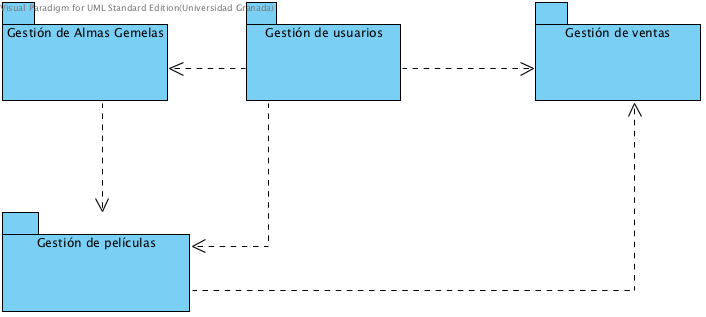
\includegraphics[width=0.9\textwidth]{Paquetes.png}
  \caption{Diagrama de paquetes}
\end{center}
\end{figure}

\section{Diagrama de casos de uso}
\section{Descripción básica de casos de uso}


%======================================
%Ejemplo de tabla de casos de uso:
%======================================
\begin{table}[h]
\begin{tabular}{|l|l|l|l|l|l|}
\hline
\multicolumn{2}{|p{2cm}|}{Casos de uso}  & \multicolumn{3}{p{7cm}|}{} & CU-x \\
\hline
\multicolumn{2}{|p{2cm}|}{Actores}       & \multicolumn{4}{p{8cm}|}{}        \\
\hline
\multicolumn{2}{|p{2cm}|}{Tipo}          & \multicolumn{4}{p{8cm}|}{}        \\
\hline
\multicolumn{2}{|p{2cm}|}{Precondición}  & \multicolumn{4}{p{8cm}|}{}        \\
\hline
\multicolumn{2}{|p{2cm}|}{Postcondición} & \multicolumn{4}{p{8cm}|}{}        \\
\hline
\multicolumn{6}{|p{10cm}|}{Proposito}                                   \\
\hline
\multicolumn{6}{|p{10cm}|}{}                                            \\
\hline
\multicolumn{6}{|p{10cm}|}{Descripción}                                 \\
\hline
\multicolumn{6}{|p{10cm}|}{}                                            \\
\hline
Autor              &              & Fecha    &     &   Versión  &\\     
\hline
\end{tabular}
\end{table}


\end{document}
